\documentclass{article}
\usepackage[utf8]{inputenc}
\usepackage{caption}
\usepackage{amsmath}
\usepackage{amssymb}
\usepackage{mathtools}
\usepackage{multicol}
\usepackage{graphicx}
\usepackage{wrapfig}
\usepackage{float}
\usepackage[makeroom]{cancel}
\usepackage{mhchem}
\usepackage{pst-plot}

\graphicspath{ {../images/} }

\renewcommand{\familydefault}{\sfdefault}
\renewcommand{\baselinestretch}{1.5} % line spacing
\newcommand{\fline}{\par\noindent\rule{\textwidth}{0.1pt}} % horizontal line (wide)

\title{Topic 9 Acids \& Bases\\Lesson 2 - Oxidizing + Reducing Agents}
\author{Peter Zhang}

\begin{document}

\maketitle
\tableofcontents
\newpage

% lesson 
\section{REDOX Agents}
\begin{itemize}
\item Reactants that \textbf{accept} \ce{e-} are oxiding agents (oxidant)\\They undergo reduction\\Non-metals due to greater EN
\item Reactants that \textbf{supply} \ce{e-} are reducing agents (reductant)\\They undergo \textbf{oxidation}\\Metals
\end{itemize}

Stronger the reduction agent the easier it is to remove \ce{e-}\\\textbf{oxidation loses \ce{e-}} + \textbf{reducing gains \ce{e-}}\\\textbf{THE OXIDANT is being reduced and the REDUCTANT is being oxidized}


COLOR DIF = TRANSITION METAL OXIDATION CHANGE

\begin{figure}[H]
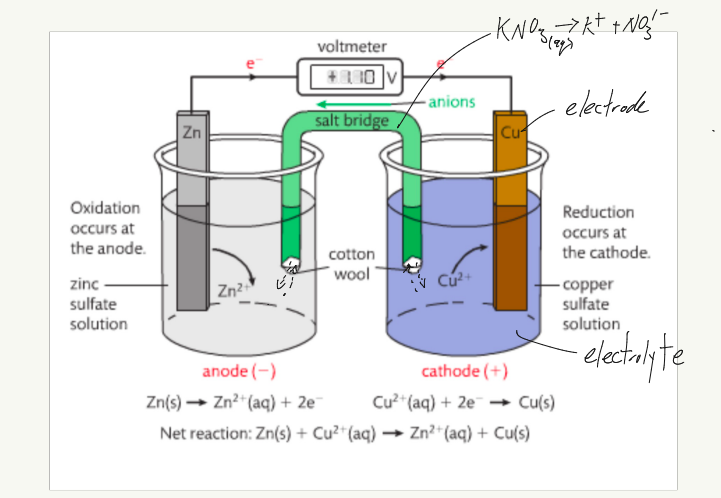
\includegraphics[width=\textwidth]{5.2circuit.png}
\captionof{figure}{Circuit Setup}
\end{figure}








\end{document}